\documentclass[a4paper,12pt]{article}
\usepackage[italian]{babel}
\usepackage{geometry}
\usepackage{fancyhdr}
\usepackage[T1]{fontenc}
\usepackage[utf8]{inputenc}
\pagenumbering{arabic}
\usepackage{lmodern}
\usepackage{graphicx}
\usepackage[export]{adjustbox}
\usepackage{xcolor}
\usepackage{setspace}
\usepackage{booktabs}
\usepackage{amsmath}
\usepackage{subcaption}
\usepackage{enumitem}
\usepackage{amsmath}
\usepackage{afterpage}
\usepackage{tabularx}
\usepackage{multirow}
\usepackage{float}
\usepackage{wrapfig}

\usepackage{epigraph}
\usepackage{pdfpages}
\usepackage{ragged2e}
\usepackage[version=3]{mhchem}

\usepackage[backend=bibtex, sorting=none]{biblatex}

\addbibresource{Bibliografia.bib}

\begin{document}


	\begin{titlepage}
	
	\end{titlepage}
	\newpage        
	\tableofcontents                        
	\clearpage\null\thispagestyle{empty}\newpage
	

	\section{Introduzione}

\subsection{Obiettivi}
Lo scopo dell'esperienza è lo studio della regione del Cigno, con particolare attenzione all'analisi dello spettro di emissione dell'idrogeno neutro $\textbf{HI}$, andando a soffermarci sulla riga 21 cm. 
In ultima analisi verrà compiuta una mappa della regione di cielo osservata, per evidenziare la distribuzione spaziale dell'idrogeno.
\\\\
Per condurre tale esperimento sarà utilizzata la strumentazione universitaria, parabola e ricevitore, opportunamente calibrata.
\\\\
Di seguito verrà esposta una breve trattazione teorica, a cui seguirà una descrizione accurata dell'apparato strumentale. Passando poi a descrivere la calibrazione della parabola e del ricevitore, la quale è necessaria per l'effettiva analisi dati e mappatura della regione. Infine riassumeremo i risultati ottenuti nella conclusione.



\subsection{Sorgente}
La sorgente galattica di interesse è il Cigno, individuabile attraverso le coordinate celesti, ascensione retta e declinazione, pari a RA $\sim$ 308 deg e Dec $\sim$ 42 deg.
Studiando il flusso, ovvero radiazione di natura elettromagnetica, rilevato in funzione della frequenza si ottiene lo spettro caratteristico della sorgente. Quest'ultimo è ascrivibile a tre componenti distinte: 
\begin{itemize}
\item Spettro di emissione, spettro discreto con linee di emissione a determinate frequenze;
\item Spettro d'assorbimento, spettro discreto con linee d'assorbimento a determinate frequenze;
\item Spettro continuo causato dall'emissione a tutte le frequenze, dovuto al comportamento della sorgente assimilabile a un corpo nero a una data temperatura. 
\end{itemize}

\subsubsection*{Spettro di emissione}
L'origine dello spettro di emissione è il fenomeno dell'eccitamento e il conseguente diseccitamento degli elettroni negli atomi. La radiazione osservata è l'emissione di fotoni con un'energia prossima al salto energetico compiuto.

\begin{figure}[h]
\includegraphics[scale=0.30]{transizione.pdf}
\centering
\caption{Rappresentazione schematica delle transizioni all'interno di un atomo di idrogeno}
\end{figure}


\subsubsection*{Spettro di assorbimento}
Lo spettro di assorbimento è imputabile a un mezzo, solitamente a temperatura minore della sorgente, interposto tra essa e l'osservatore. I fotoni emessi dalla sorgente primaria eccitano atomi nel mezzo, a loro volta diseccitandosi emettono fotoni casualmente in ogni direzione, dando luogo all'assenza di righe nello spettro.


\subsubsection*{Spettro continuo}
A generare lo spettro continuo concorrono due principali fenomeni: 
\begin{itemize}
\item Radiazione termica, a sua volta distinguibile in bremsstrahlung, corpo nero e polvere interstellare;
\item Radiazione non termica, emissione di sincrotone. 
\end{itemize}

In particolar modo, il fenomeno del bremsstrahlung è dovuto al rallentamento di un elettrone libero all'interno dell'atomo, essendo una particella carica in decelerazione emette fotoni in modo continuo. Particolarmente diffuso in regione con HII, ovvero nubi di idrogeno ionizzato da raggi ultravioletti associati a stelle nascenti o morenti.
\\\\
La nube di idrogeno è a una data temperatura, per tale motivo emette radiazione con uno spettro assimilabile a un copro nero, piccando a una sua temperatura caratteristica. 
\\\\
La polvere interstellare assorbe luce stellare in banda ottica, aumento la propria temperatura. Tale aumento comporta emissione termica in banda infrarossa.
\\\\
Per quanto concerne la radiazione di sincrotone, essa è dovuta all'emissione di fotoni da parte di elettroni in moto variabile all'interno del campo magnetico galattico. Lo spettro è tipico di un corpo grigio\cite{Gervasi22:Dispensa}.


\subsection{Riga idrogeno}
Il soggetto principale dello studio è la riga a 21 cm dell'idrogeno neutro. Prende tale nome dalla lunghezza d'onda a cui si manifesta 21,10611405413 cm, corrispondenti a 1420,405 MHz, nella banda delle microonde. La transizione avviene tra due stati iperfini, come riportato in figura \ref{fig:Iperfine}, a causa di uno spin flipping, ovvero transizione da uno stato in cui $e^{-}$ e $p^{+}$ hanno spin parallelo ad uno stato in cui $e^{-}$ e $p^{+}$ hanno spin antiparallelo. La struttura iperfine si ottiene considerando i termini di interazione tra: il momento magnetico del protone e il campo generato dall'elettrone, dipolo-dipolo magnetico tra $e^{-}$ e $p^{+}$, e momento magnetico di $e^{-}$ col campo magnetico interno al $p^{+}$\cite{Cohen:libro}.
Il decadimento è estremamente proibito e il tempo di vita medio per tale stato eccitato è dell'ordine di $\tau \simeq 10 ^{7}$  anni\cite{Mhaske:articolo}.
Nonostante tale caratteristica è possibile osservare la transizione  a causa dell'elevato numero di atomi di H nella regione di analisi, pur considerando una densità bassa pari a $\simeq$ 100 $\frac{atomi}{cm^{3}}$. 


\begin{figure}[h]
\includegraphics[scale=0.18]{Iperfine.pdf}
\hfill
\includegraphics[scale=0.18]{Flipping.pdf}
\centering
\caption{Rappresentazione della struttura iperfine, spin flipping della transizione che genera la riga 21}
\label{fig:Iperfine}
\end{figure}


	\section{Apparato Sperimentale}



\subsection{Parabola}

\begin{wrapfigure}{r}{0.25\textwidth}
    \centering
    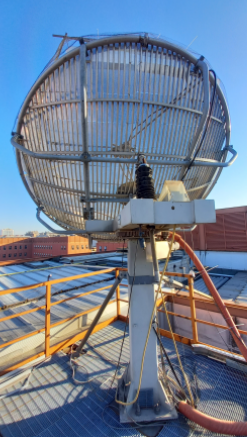
\includegraphics[width=0.25\textwidth]{Parabola.png}
    \caption{Parabola Bicocca}
\end{wrapfigure}

Lo strumento utilizzato per la ricezione del segnale è un telescopio riflettore, ovvero un'antenna radio di forma parabolica, il cui diametro è di 3 m. Nel punto focale sono situati i ricevitori, tre analogici e uno digitale.
I ricevitori analogici lavorano a diverse frequenze, 1,4; 2,5; 10 GHz. A sua volta il ricevitore digitale presenta due porte di ingresso, una a 1,4 GHz e una a 2,5 GHz.
In particolare, nella seguente analisi verrà utilizzato la porta a 1,4 GHz del ricevitore digitale.
\\\\
Per muovere la parabola nella regione di cielo di interesse, vengono inseriti, sul software, i valori di azimuth, elevazione e orario di puntamento. Per quanto concerne l'azimuth, è da tener conto l'off-set dovuto alla posizione del ricevitore. Nel caso in esame l'off-set corrisponde ad un angolo di 21.0 gradi. 

\subsection{Ricevitore digitale}
La larghezza di banda del ricevitore è di 160 MHz, permettendo così un'analisi in un range di $\nu \in$  [1,30;1,46] GHz. Sono presenti 8192 canali, ciascuno con una larghezza di banda pari a $\Delta\nu$ = 19531,25 Hz \cite{Canali:canali}.%non funziona la citazione
\\\\
La velocità di campionamento della radio è di 160 Msamples/s, la media temporale è eseguita su 320 Msamples spaziando un intervallo di circa 2 secondi. Tale media permette di ottenere un dato sufficientemente sensibile a variazioni dell'ordine del secondo, oltre a ridurre sensibilmente il rumore. 


\subsection{Organizzazione file}
Le misure vengono salvate su un unico file dopo aver collezionato 150 record. Ogni file corrisponde a un tempo di presa dati di circa 5 minuti.
\\\\
I file, restituiti dal ricevitore digitale, sono organizzati nella seguente modalità. In ciascun record, i primi tre valori corrispondono rispettivamente a:
\begin{itemize}
\item tempo: tempo trascorso dall'apertura del file espresso in millisecondi;
\item frequenza: frequenza del canale a frequenza più bassa espressa in Hz;
\item frequency step: step in frequenza tra due canali successivi, espresso in Hz.
\end{itemize}
Le entrate successive, espresse in dBm, corrispondono al segnale registrato dal ricevitore, ripetuto per ognuno degli 8192 canali.
\\\\
Nell'analisi sono anche utilizzati i file della parabola, da cui si ricavano i valori di temperatura del cavo che connette la parabola al ricevitore. %capire ricevitore/elaboratore


\subsection{Programma coordinate}
\label{Programma coordinate}
Dato un orario di osservazione, per determinare le coordinate a cui porre la parabola, viene utilizzata la libreria astropy. In particolare la funzione che implementa il cambio di coordinate da celesti ad azimuth ed elevazione è \textit{transform to}.  Necessario conoscere i valori di longitudine, latitudine ed elevazione rispetto al livello del mare del luogo in cui è situata la parabola, i.e. Milano. Inoltre bisogna tener conto della regione UTC, per settare correttamente l'offset. 

\begin{figure}[h]
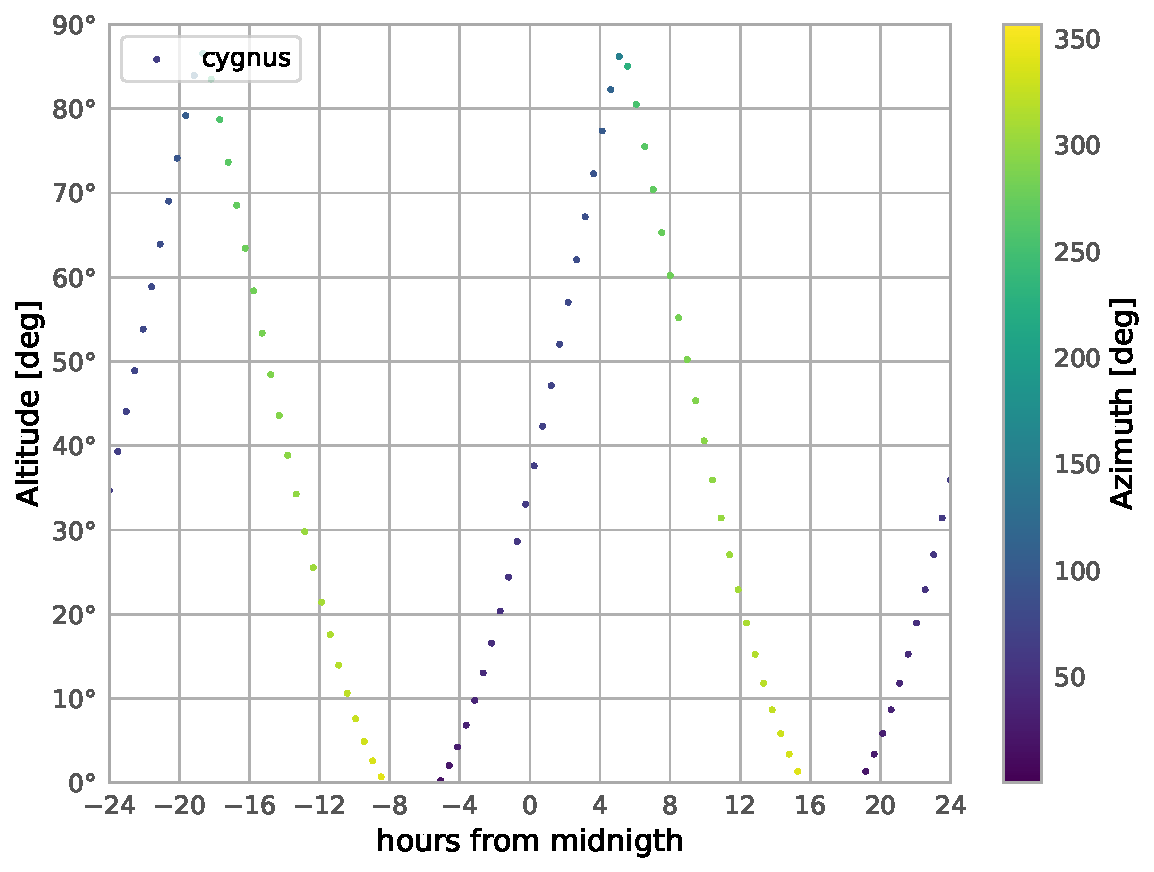
\includegraphics[scale=0.60]{Coordinate.pdf}
\centering
\caption{L'immagine mostra la traiettoria della sorgente in un arco di 48 ore.}
\label{fig:Coordinate}
\end{figure}

	\section{Calibrazione}
La calibrazione del ricevitore a 1.4 a GHz viene effettuata utilizzando due sorgenti di riferimento, che sono due carichi coassiali adattati, cioè due resistenze a 50 $\Omega$. Questi lavorano a due temperature diverse: uno a temperatura ambiente (\textit{warm load}) e l'altro alla temperatura di ebollizione dell'azoto liquido, ovvero 77,36 K (\textit{cold load}). \\\\Il carico a temperatura criogenica è connesso al ricevitore tramite un cavo coassiale il quale è immerso parzialmente nell'azoto liquido. Perciò, dato che la temperatura del cavo non è uniforme, ne vanno studiate le caratteristiche di attenuazione in laboratorio, su un cavo analogo, a temperatura ambiente ed a temperatura criogenica. Per farlo si utilizza un analizzatore vettoriale di reti (VNA).

\subsection{Attenuazione cavo coassiale}
Il cavo Cold Load che viene utilizzato nella calibrazione del ricevitore è solo parzialmente immerso nell'azoto liquido, la sua temperatura non è quindi costante. Perciò, il coefficiente di attenuazione del cavo viene misurato con il VNA sia a temperatura ambiente, sia a temperatura criogenica. Per farlo si utilizza un cavo di rame analogo di forma elicoidale, così da facilitarne l'immersione nell'azoto, e di lunghezza 203 cm. 

\begin{figure}[h]
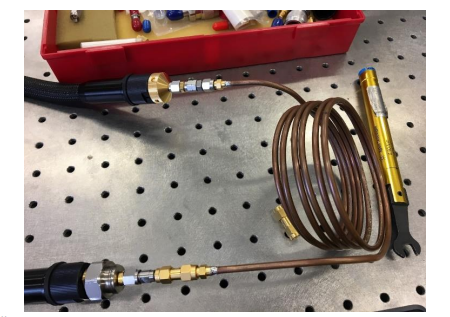
\includegraphics[scale=0.60]{cavo rame.png}
\centering
\caption{Cavo di rame collegato alle porte del VNA}
\label{fig:Cavo di rame}
\end{figure}

Il rame, però, ha una conducibilità termica molto elevata. Per questo motivo, al fine di prottegere il VNA ed evitare che i suoi cavi lavorino ad una temperatura di 77,36 K, si utilizzano dei separatori termici. Essi stessi tuttavia attenuano il segnale. Viene quindi effettuata una misura intermedia dell'attenuazione dei separatori, collegandoli tra loro. In questo modo è poissibile togliere il loro contributo dal calcolo del coefficiente di attenuazione del cavo di rame.

\subsubsection{VNA e parametri di scattering}
Il VNA è una macchina che permette di misurare le proprietà di trasmissione di un cavo coassiale i cui estremi sono connessi ai terminali dello strumento. Il VNA presente il laboratorio è un Agilent PNA-X che è in grado di misurare in modo indipendente il segnale di trasmissione e riflessione dalle due porte presenti.
\begin{figure}[h]
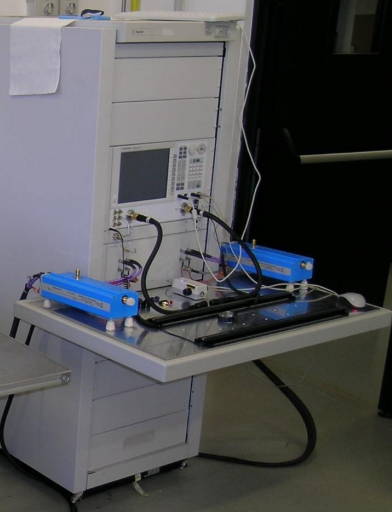
\includegraphics[scale=0.60]{VNA.png}
\centering
\caption{VNA presente in laboratorio. Il modello è un Agilent PNA-X.}
\label{fig:VNA}
\end{figure}

Quindi ciò che la macchina restituisce è la cosiddetta matrice di scattering i cui parametri sono: i coefficienti di riflessione, \textit{$s_{11}$} e \textit{$s_{22}$}, ed i coefficienti di trasmissione, \textit{$s_{12}$} e \textit{$s_{21}$}. Dove vale che:\\\\
\begin{equation}
    s_{11}=10\log_{10} \frac{Potenza\,\,riflessa\,\,nella\,\,porta\,\,1}{Potenza\,\,incidente\,\,dalla\,\,porta\,\,1},
\end{equation}
\begin{equation}
    s_{12}=10\log_{10} \frac{Potenza\,\,trasmessa\,\,dalla\,\,porta\,\,1\,\,alla\,\,porta\,\,2}{Potenza\,\,incidente\,\,dalla\,\,porta\,\,1},
\end{equation}
\begin{equation}
    s_{21}=10\log_{10} \frac{Potenza\,\,trasmessa\,\,dalla\,\,porta\,\,2\,\,alla\,\,porta\,\,1}{Potenza\,\,incidente\,\,dalla\,\,porta\,\,2},
\end{equation}
\begin{equation}
    s_{22}=10\log_{10} \frac{Potenza\,\,riflessa\,\,nella\,\,porta\,\,2}{Potenza\,\,incidente\,\,dalla\,\,porta\,\,2};
\end{equation}



\subsubsection{Matrice di scattering con separatori termici}
\label{ssec:Matrice di scattering con separatori termici}

I separatori termici vengono connessi tra loro tramite degli adattatori, attraverso tale processo è possibile ricavare i coefficienti di trasmissione, $ s_{21} $, e riflessione, $ s_{11} $, a temperatura ambiente e temperatura criogenica, rispettivamente $ T_{A}\sim290K $ e $ T_{C} = 77.36K $. Più dettagliatamente:

\begin{itemize}
\item s11: si instaurano onde stazionarie durante il percorso. Sono presenti dei minimi e dei massimi, quindi a determinare lunghezze d'onda il segnale avrà riflessione massima o minima, ma comunque inferiore all'1 \% del segnale;
\item s21: anche in questo caso sono presenti oscillazioni, con un'attenuazione di 0.4 dB.
\end{itemize}

\begin{figure}[H]
\centering

\begin{subfigure}{0.49\textwidth}
	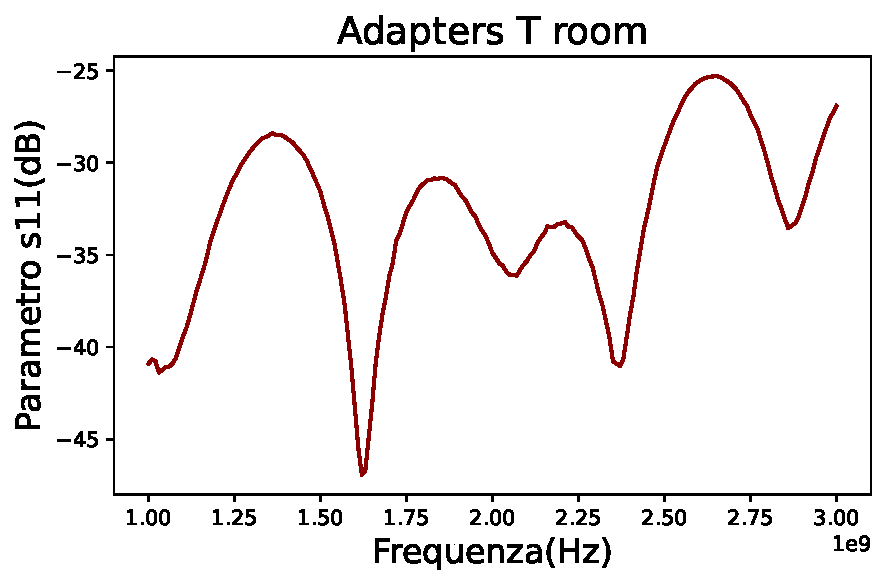
\includegraphics[width=\textwidth]{S11_TA.pdf}
    \caption{$s_{11}$ separatori termici a $T_{A}$}
    \label{fig:sub1}
\end{subfigure}
\hfill
\begin{subfigure}{0.49\textwidth}
    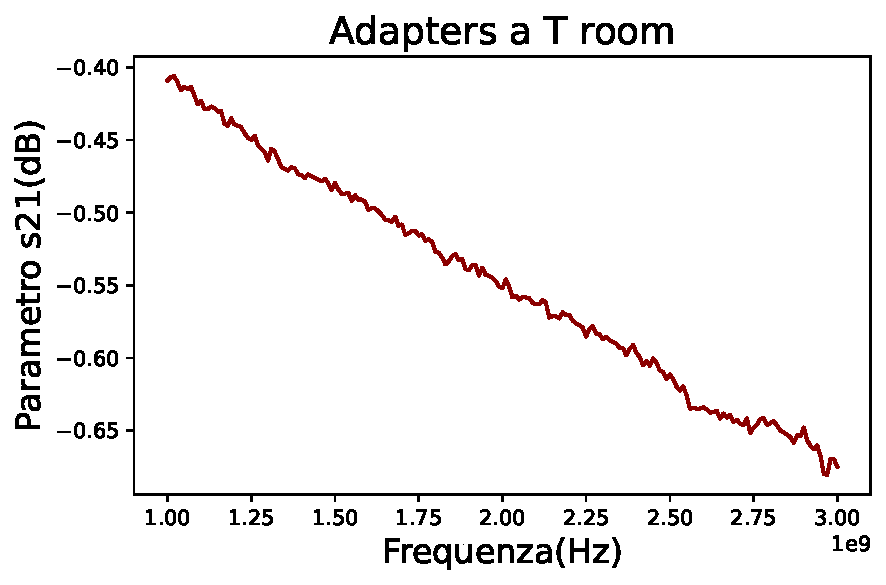
\includegraphics[width=\textwidth]{S21_TA.pdf}
    \caption{$s_{21}$ separatori termici a $T_{A}$}
    \label{fig:sub2}
\end{subfigure}

\end{figure}

\begin{figure}[H]
\centering

\begin{subfigure}{0.49\textwidth}
	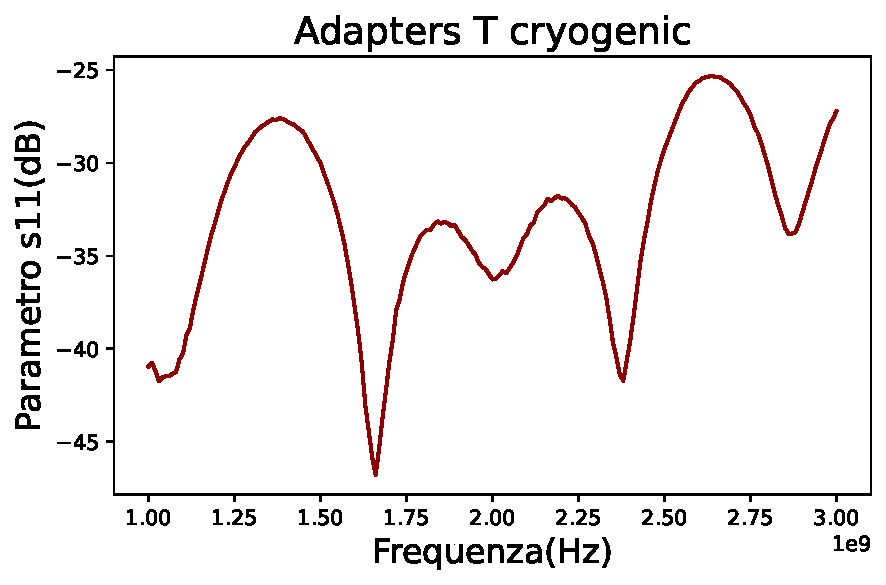
\includegraphics[width=\textwidth]{S11_TC.pdf}
    \caption{$s_{11}$ separatori termici a $T_{C}$}
    \label{fig:sub1}
\end{subfigure}
\hfill
\begin{subfigure}{0.49\textwidth}
    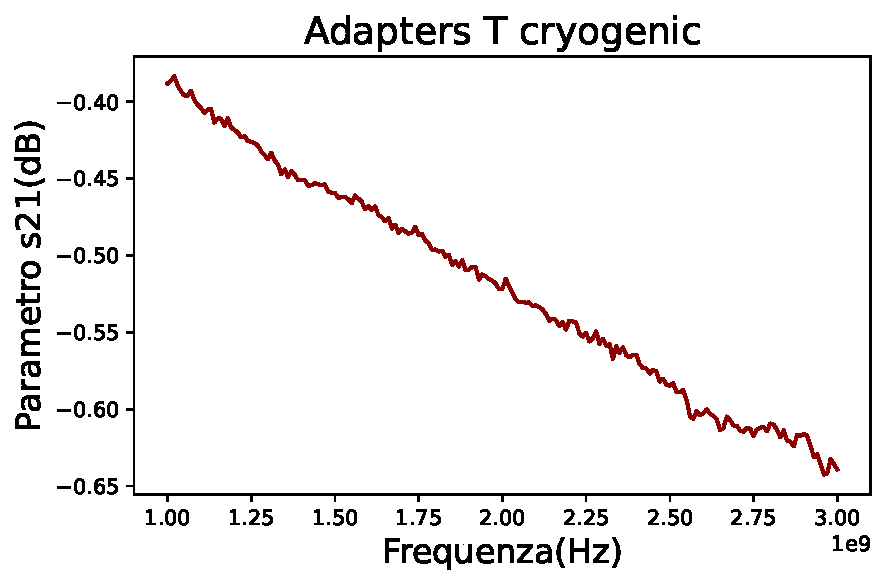
\includegraphics[width=\textwidth]{S21_TC.pdf}
    \caption{$s_{21}$ separatori termici a $T_{C}$}
    \label{fig:sub2}
\end{subfigure}

\end{figure}

\subsubsection{Matrice di scattering con separatori termici e cavo di rame}
\label{ssec:Matrice di scattering con separatori termici e cavo di rame}

Ora, i separatori termici vengono collegati al cavo di rame e ripetute le misure sia a temperatura ambiente, sia a temperatura criogenica immergendoli in azoto liquido.

\begin{figure}[H]
\centering

\begin{subfigure}{0.49\textwidth}
	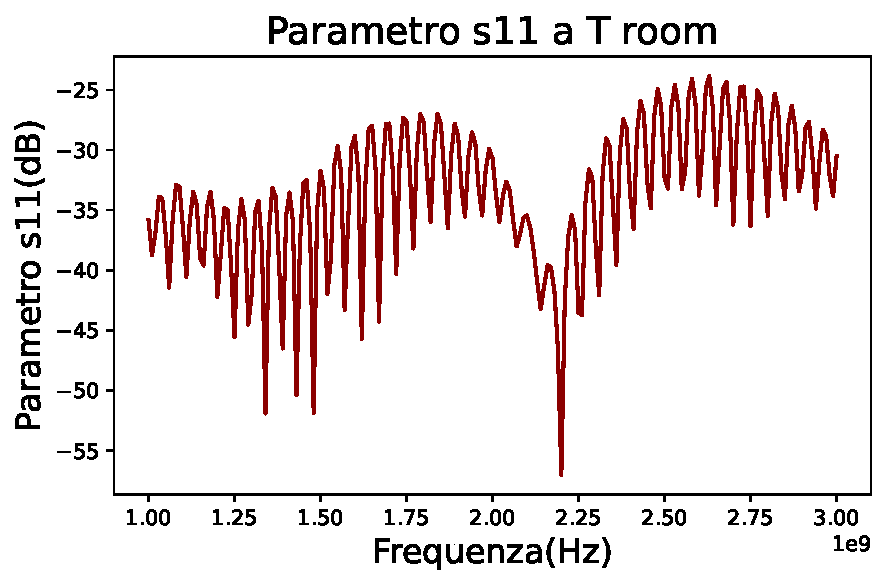
\includegraphics[width=\textwidth]{S11_TA_rame.pdf}
    \caption{$s_{11}$ separatori termici e rame a $T_{A}$}
    \label{fig:sub1}
\end{subfigure}
\hfill
\begin{subfigure}{0.49\textwidth}
    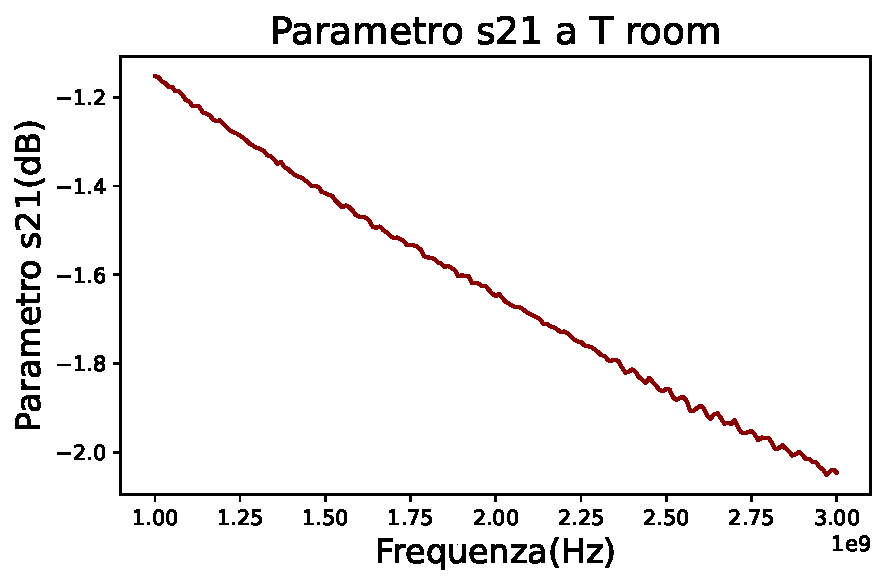
\includegraphics[width=\textwidth]{S21_TA_rame.pdf}
    \caption{$s_{21}$ separatori termici e rame a $T_{A}$}
    \label{fig:sub2}
\end{subfigure}

\end{figure}

\begin{figure}[H]
\centering

\begin{subfigure}{0.49\textwidth}
	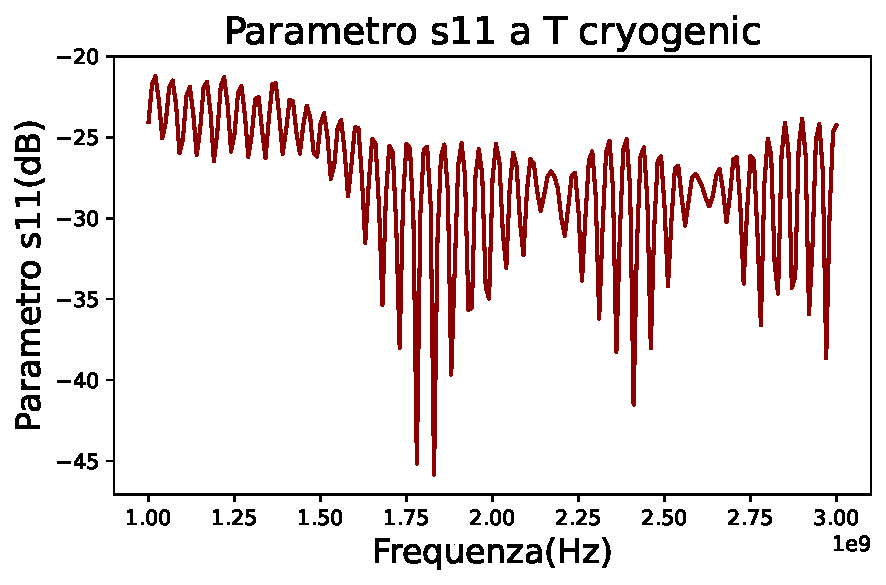
\includegraphics[width=\textwidth]{S11_TC_rame.pdf}
    \caption{$s_{11}$ separatori termici e rame a $T_{C}$}
    \label{fig:sub1}
\end{subfigure}
\hfill
\begin{subfigure}{0.49\textwidth}
    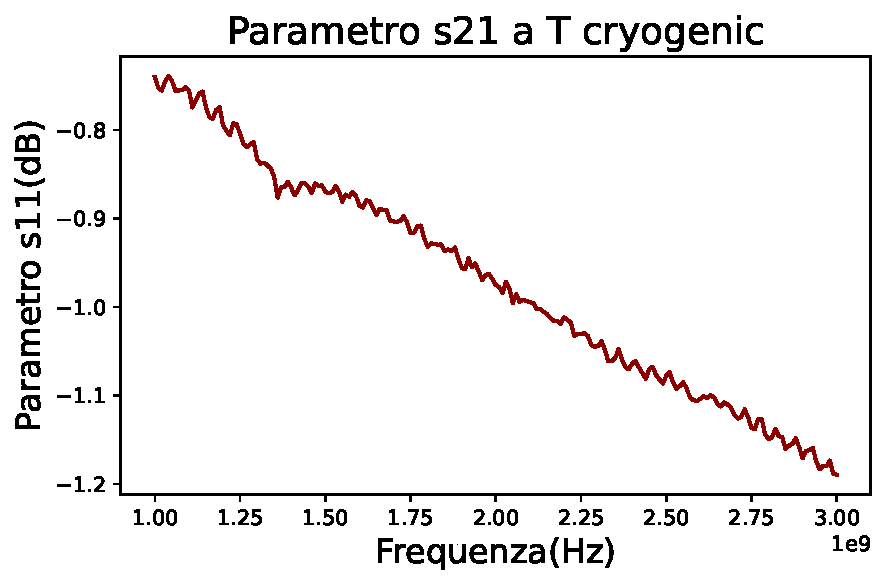
\includegraphics[width=\textwidth]{S21_TC_rame.pdf}
    \caption{$s_{21}$ separatori termici e rame a $T_{C}$}
    \label{fig:sub2}
\end{subfigure}

\end{figure}

\`E possibile notare un incremento delle oscillazione, infatti l'aumento della lunghezza complessiva porta a un numero maggiore di onde stazionarie; la variazione complessiva tra massimo e minimo rimane comunque di 20 dB.


\subsubsection{Matrice di scattering del cavo di rame}
\label{ssec:Matrice di scattering del cavo di rame}

Ottenuti gli andamenti nelle due configurazioni, descritte in \ref{ssec:Matrice di scattering con separatori termici e cavo di rame} e \ref{ssec:Matrice di scattering con separatori termici}, si può sottrarre il contributo dei separatori e ottenere infine il coefficiente di trasmissione $s_{21}$ per il solo cavo di rame. Viene riportato di seguito l'andamento di tale valore in funzione della frequenza, sia a $ T_{A}\sim290K $, sia a $ T_{C} = 77.36K $.

\begin{figure}[H]
\centering

\begin{subfigure}{0.49\textwidth}
	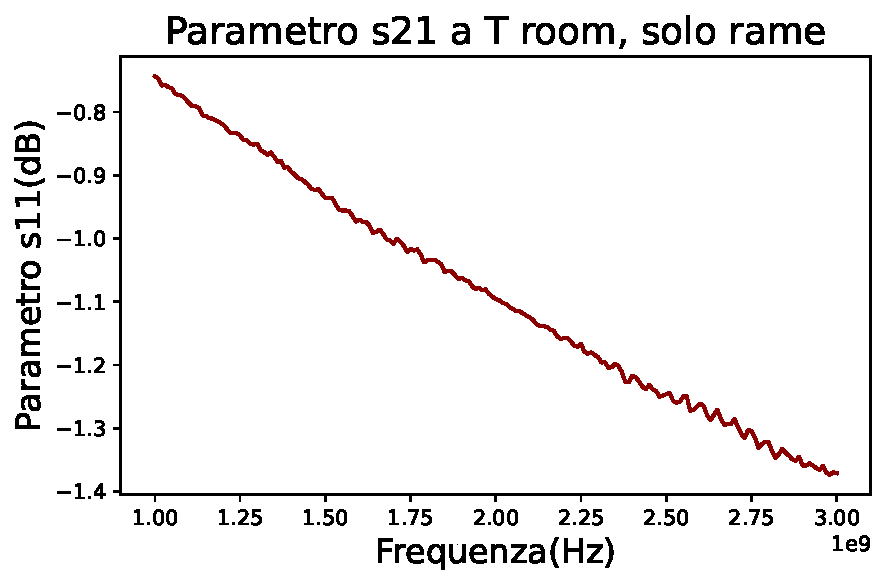
\includegraphics[width=\textwidth]{S21_TA_solo_rame.pdf}
    \caption{$s_{21}$ solo rame a $T_{A}$}
    \label{fig:sub1}
\end{subfigure}
\hfill
\begin{subfigure}{0.49\textwidth}
    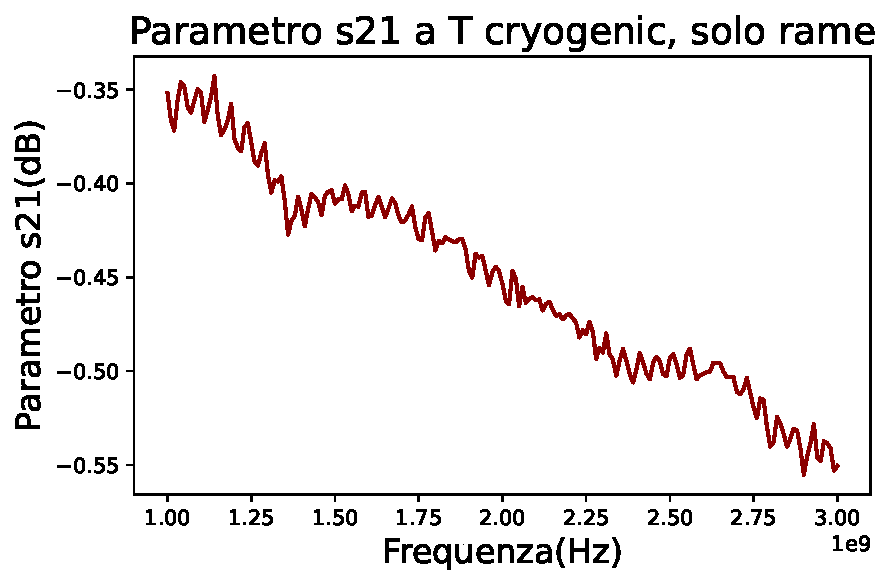
\includegraphics[width=\textwidth]{S21_TC_solo_rame.pdf}
    \caption{$s_{21}$ solo rame a $T_{C}$}
    \label{fig:sub2}
\end{subfigure}
\caption{Parametri di trasmissione del solo cavo di rame}
\label{fig:Solo_rame}
\end{figure}



\subsubsection{Coefficiente di attenuazione}
\label{ssec:Coefficiente di attenuazione}

Bisogna ora calcolare il coefficiente di attenuazione $\tau$ del cavo alla frequenza della riga HI. Per farlo valutiamo il coefficiente di trasmissione $\alpha$ = $e^{-\tau}$. Però, dato che la temperatura del cavo non è costante, è più opportuno ricavare il coefficiente di trasmissione per unità di lunghezza e in funzione della temperatura. Assumendo ora che le perdite ohmiche nel metallo siano dominanti rispetto alle perdite nel dielettrico del cavo (approssimazione ben valida), possiamo dire che il coefficiente di trasmissione espresso in potenza è direttamente proporzionale alla resistività $\rho$ del metallo (il campo elettrico va come $\sqrt{\rho}$). Questa, inoltre, è proporzionale alla temperatura secondo la seguente relazione:

\begin{equation}
    \rho(T)=\rho_{0}+\alpha[T-T_{0}].
\end{equation}

Ora, la potenza in uscita dal cavo è data da:

\begin{equation}
    P_{out}=P_{in}(1-R)\alpha,
    \label{potenza}
\end{equation}

dove R e $\alpha$ sono rispettivamente i coefficienti di riflessione e trasmissione espressi in scala lineare. 
Il VNA, invece, restituisce un valore di $\alpha_{eff}$, dato da $P_{out}=\alpha_{eff}P_{in}$ ed espresso in db:

\begin{equation}
    \alpha_{eff}=10\log_{10}\frac{P_{out}}{P_{in}}=s_{21}.
\end{equation}

Se teniamo in considerazione l'equazione \eqref{potenza} e che R[db] 
=  $s_{11}$, allora si ottiene:

\begin{equation}
    \alpha=\frac{10^{\frac{\alpha_{eff}[db]}{10}}}{1-R}=\frac{10^{\frac{s_{21}[db]}{10}}}{1-10^{\frac{s_{11}[db]}{10}}}\simeq10^{\frac{s_{21}[db]}{10}},
\end{equation}

dove è stato possibile compiere l'ultima approssimazione dato che il valore di $s_{11}$ è minore di 20 db, cioè si ha una correzione al coefficiente di trasmissione minore dell'1$\%$.\\
Infine, sapendo che $\alpha = e^{-\tau x}$, dove x è la lunghezza del cavo, possiamo ricavare $\tau$ da:

\begin{equation}
    \tau=-\frac{\ln{\alpha}}{x}.
\end{equation}

\subsubsection{Verifica andamento lineare}
\label{ssec:Verifica andamento lineare}
Essendo noti i valori di $s_{21}$ a $ T_{A}\sim290K $ e $ T_{C} = 77.36K $, e di conseguenza i corrispettivi valori del coefficiente di attenuazione a suddette temperature; per ricavare il valore di $ \tau $ ad ogni temperatura, viene eseguita un'interpolazione con una retta. Per verificare che l'andamento sia effettivamente lineare, ci si avvale di un valore teorico, ricavato dal grafico in figura \ref{fig:Tre_punti} ,a $ T \sim4,2K $,  $ \tau \sim 4\cdot  10^{-5}  Neper/mm$.

\begin{figure}[H]
	\centering
	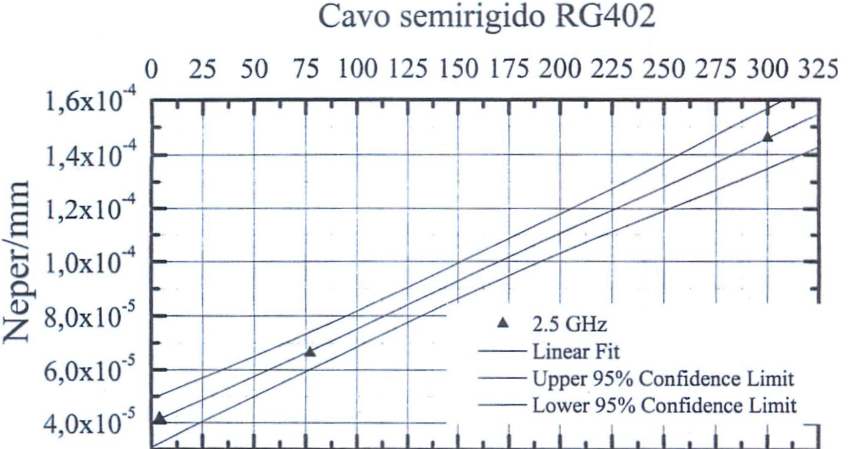
\includegraphics[scale=0.8]{Tre_punti.png}
	\caption{Tau vs Temperatura a 2.5 GHz}
    	\label{fig:Tre_punti}
\end{figure}

I valori di $s_{21}$ alla frequenza di interesse sono ricavati dai plot in figura \ref{fig:Solo_rame},  tramite la funzione interp della libreria numpy di python. Tale funzione, assegnato un set discreto di dati come frequenze e $s_{21}$, restituisce il valore a un dato x-value richiesto, eseguendo un'interpolazione lineare. Tale procedura è necessaria in quanto il set di dati discreto non presenta il valore esattamente a 2,5 GHz. Vengono riportati in tabella i valori finali:

\begin{table}[h!]
\centering

\begin{tabular}{ |c|c|  }
	\hline
	\multicolumn{2}{|c|}{$\tau $ ricavati a 2.5 GHz} \\
	\hline
	Temperatura (K)& $\tau\cdot  10^{-5}$ (Neper/mm) \\
	\hline
	4,2   &  4,0   \\
	77,36  & 5,6 \\
	290 &14,1 \\
	\hline
\end{tabular}

\end{table}


\begin{figure}[H]
	\centering
	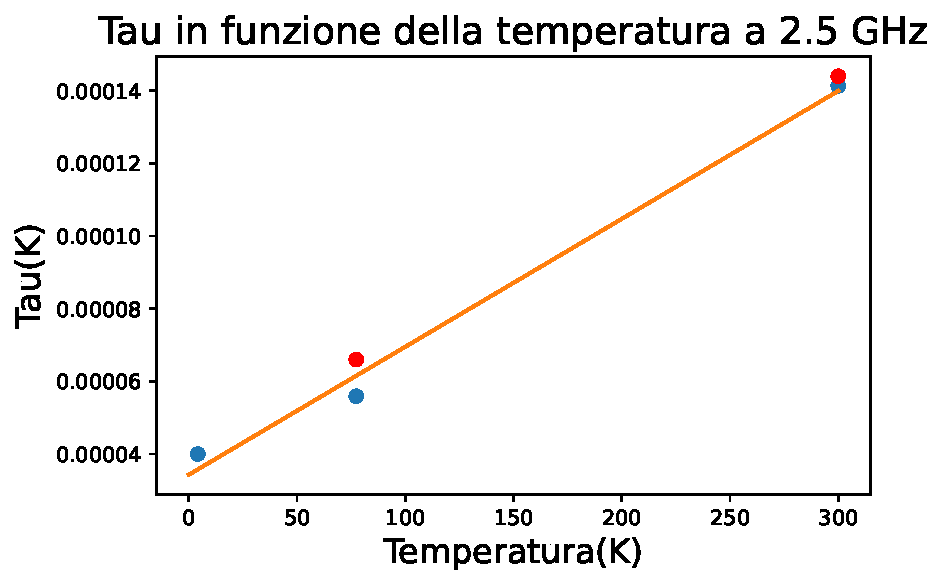
\includegraphics[scale=0.8]{Tau_Temp_2,5.pdf}
	\caption{I punti in blu sono i valori riportati in tabella, i due punti rossi sono la rappresentazione dei restanti punti del grafico in figura \ref{fig:Tre_punti}, mostrati per vedere quanto si discostassero dai punti sperimentali}
    	\label{fig:Tau_2,5}
\end{figure}

Dal grafico in figura \ref{fig:Tau_2,5}, si evince chiaramente un andamento lineare che si può estendere al caso di 1,4 GHz.

\subsubsection{Calcolo coefficiente a 1.4 GHz}
\label{ssec:Calcolo coefficiente a 1.4 GHz}

Viene rieseguita la procedura descritta in \ref{ssec:Verifica andamento lineare}, applicata al caso 1.4 GHz. Si ottengono i seguenti risultati: 

\begin{table}[H]
\centering

\begin{tabular}{ |c|c|  }
	\hline
	\multicolumn{2}{|c|}{$\tau $ ricavati a 1.4 GHz} \\
	\hline
	Temperatura (K)& $\tau\cdot  10^{-5}$ (Neper/mm) \\
	\hline
	77,36  & 4,7 \\
	290 &10,3 \\
	\hline
\end{tabular}

\end{table}


\begin{figure}[H]
	\centering
	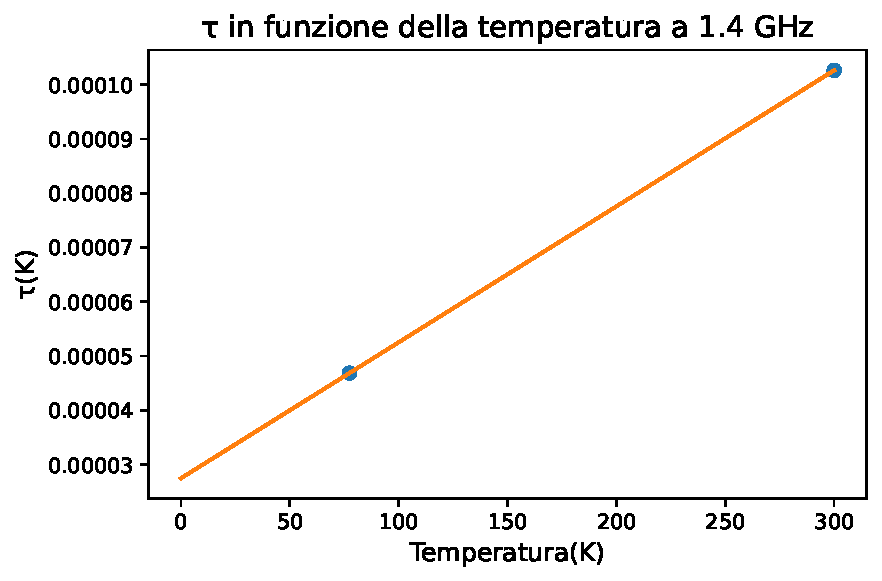
\includegraphics[scale=0.8]{Tau_Temp_1,4.pdf}
	\caption{Interpolazione lineare dei $\tau$ a 1,4 GHz}
    	\label{fig:Tau_2.5}
\end{figure}



\subsection{Calibrazione del ricevitore a 1.4 GHz}

La conoscenza del profilo del coefficente di attenuazione in funzione della temperatura permette di attuare la calibrazione del ricevitore a 1,4 GHz. Si consideri come warm load e cold load, un cavo rispettivamente di lunghezza 12 m e 120 cm. Il cold load è immerso parzialmente nell'azoto liquido portando ad un'attenuazione del segnale.\\
Per ottenere il segnale effettivo letto dal ricevitore è quindi necessario considerare la variazione della temperatura all'interno del cavo.

\subsubsection{Profilo di temperatura del cavo}
\label{ssec:Profilo di temperatura del cavo}

La stima del profilo di temperatura è resa possibile grazie a 4 sensori criogenici e 2 sensori a temperatura ambiente posizionati sul cavo, come mostrato in figura \ref{fig:cavi}. 

\begin{figure}[H]
\centering

	\begin{subfigure}{0.49\textwidth}
		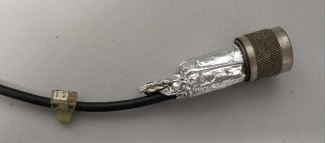
\includegraphics[width=\textwidth]{Posizione_sensori_1.png}
    		\caption{Uno dei sensori connesso al cavo warm load}
   	 	\label{fig:sub1}
	\end{subfigure}
	\hfill
	\begin{subfigure}{0.49\textwidth}
		\centering
    		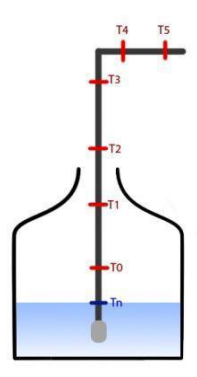
\includegraphics[width=0.5\textwidth]{Posizione_sensori_3.png}
    		\caption{Schema della posizione dei cavo durante l'immersione nell'azoto}
    		\label{fig:sub2}
	\end{subfigure}

	\begin{subfigure}{0.49\textwidth}
		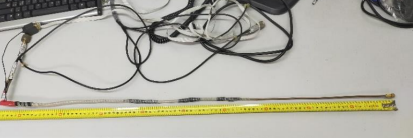
\includegraphics[width=\textwidth]{Posizione_sensori_2.png}
    		\caption{Uno dei sensori connesso al cavo warm load}
    		\label{fig:sub3}
	\end{subfigure}
	\hfill
	\begin{subfigure}{0.49\textwidth}
    		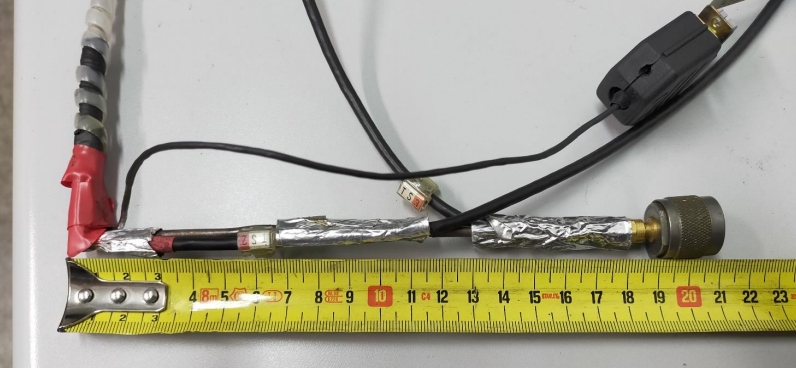
\includegraphics[width=\textwidth]{Posizione_sensori_4.png}
    		\caption{Schema della posizione dei cavo durante l'immersione nell'azoto}
    		\label{fig:sub4}
	\end{subfigure}

\caption{Visualizzazione grafica dei rilevatori sul cavo}
\label{fig:cavi}
\end{figure}


I primi 4 sensori restituiscono il valore in Kelvin, mentre gli ultimi due attuano la loro misurazione in gradi Celsius.\\
Successivamente all' immersione completa del cold load nel criostato, che contiene azoto liquido a pressione ambiente, dai valori ottenuti dai sensori è quindi possibile determinare l'andamento della temperatura in funzione della posizione: 

\begin{table}[H]
\centering

\begin{tabular}{ |c|c|  }
	\hline
	\multicolumn{2}{|c|}{Valori di temperatura registrati nella posizione del sensore} \\
	\hline
	Posizione (mm)& Temperatura (K) \\
	\hline
	295   & 77,36    \\
	380  & 110,2  \\
	480 &197,3 \\
	610    &264,3 \\
	910&   296,0  \\
	1030& 295,8  \\
	1110& 296.2  \\
	\hline
\end{tabular}

\end{table}

Infine, si fittino i seguenti valori con una funzione sigmoidale:
\begin{equation}
T= \dfrac{a}{1+e^{-k(x-x_{0})}},
\end{equation}
Il grafico che si ottiene è il seguente:

\begin{figure}[H]
	\centering
	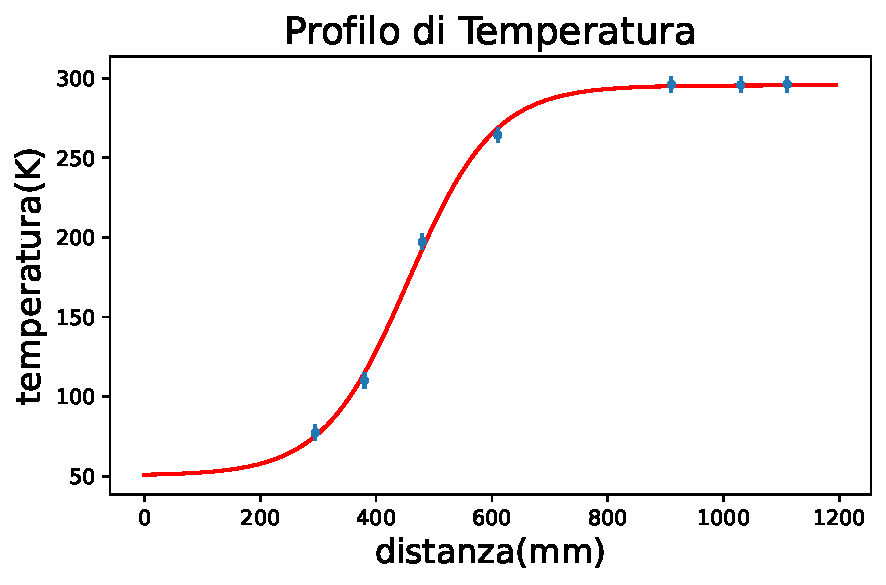
\includegraphics[scale=0.8]{Profilo_temperatura.pdf}
	\caption{Fit del profilo di temperatura}
    	\label{fig:Profilo_temperatura}
\end{figure}

Successivamente, si ricava dal profilo di  temperatura e dall'andamento del coefficiente di attenuazione in funzione della temperatura il valore di temperatura del cavo cold load e warm load.


\subsubsection{Temperatura del cavo cold load}
\label{ssec:Temperatura del cavo cold load}

L'immersione parziale del cavo cold load all'interno del criostato comporta che la temperatura del carico criogenico deve essere corretta. La propagazione della temperatura nel cavo segue il seguente andamento:

\begin{equation}
T_{b}= T_{s}e^{-\tau} + T_{C}(1-e^{-\tau}),
\label{Formula ricorsiva}
\end{equation}

dove $T_{s}$ è pari a 77,36 K, ovvero la temperatura di ebolizione dell'azoto liquido, $T_{c}$ è il valore della temperatura studiata nel paragrafo \ref{ssec:Profilo di temperatura del cavo} e $\tau$ è il coefficiente di attenuazione studiato nel paragrafo \ref{ssec:Calcolo coefficiente a 1.4 GHz}.
Si applichi tale relazione iterativamente a dei tratti di lunghezza $\Delta$x. Lo step di lunghezza viene scelto in modo tale da poter considerare il tratto di cavo preso in considerazione isotermo. Si scelga quindi un valore di $\Delta$x = 1 mm.
L'iterazione dell'equazione \eqref{Formula ricorsiva} è dovuta al fatto che il sistema risulta essere in equilibrio per tutto il tratto di cavo immerso nell'azoto liquido. \`E quindi possibile considerare valida la relazione $T_{b} = T_{s} = 77,36 K$. Nel tratto di cavo scoperto il sistema non è più all'equilibrio, la temperatura del cavo varia ed è quindi necessario determinare il coefficiente di attenuazione $\tau$ del cavo.\\
Risultante a tali considerazioni si ricava un valore di $T_{b}$ = 91,95 K.

\begin{figure}[H]
	\centering
	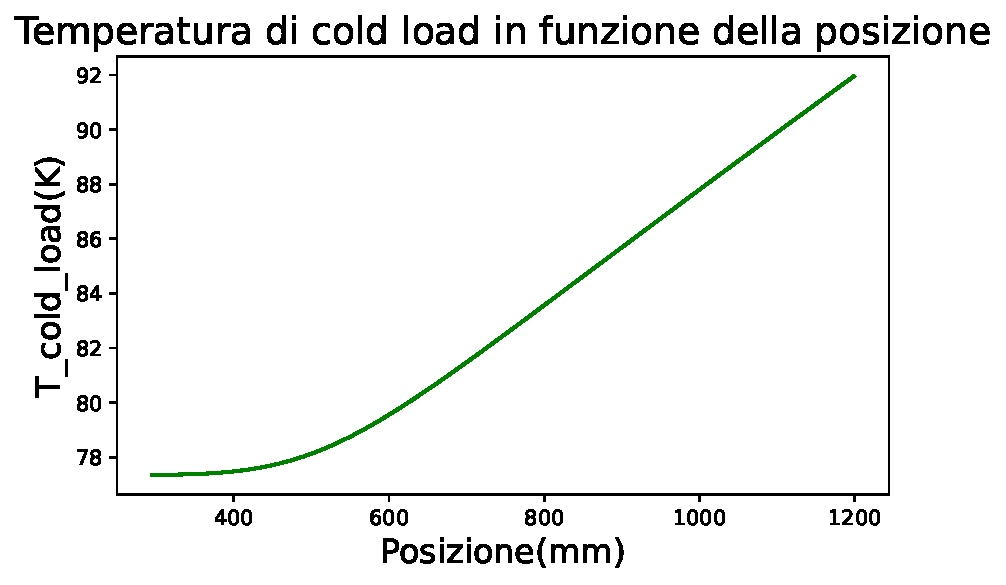
\includegraphics[scale=0.8]{Temperatura_vs_posizione.pdf}
	\caption{Andamento della temperatura di cold load in funzione della posizione}
    	\label{fig:Temperatura_vs_posizione}
\end{figure}

%\cite{Cold load:Cold load}.

\subsubsection{Temperatura del cavo warm load}
\label{ssec:Temperatura del cavo warm load}

Per determinare la temperatura del cavo warm load il procedimento è simile a quello utilizzato nel paragrafo \ref{ssec:Temperatura del cavo cold load} con la differenza che la totalità del cavo è a temperatura ambiente. Quindi la sorgente e il cavo hanno circa la stessa temperatura $T_{s}$ $\sim$ $T_{c}$ $\sim$ 294,55 K.\\
Di conseguenza risulta possibile semplificare l'equazione \eqref{Formula ricorsiva}, ottenendo come risultato per $ T_{warm} $ proprio 294,55 K.



\subsubsection{Guadagno del ricevitore}
\label{ssec:Guadagno del ricevitore}

I valori della temperatura determinati nei paragrafi \ref{ssec:Temperatura del cavo cold load} e  \ref{ssec:Temperatura del cavo warm load}  vengono utilizzati per ricavare il guadagno del ricevitore, G, e la Temperatura di rumore, $T_{R}$.\\
Il guadagno, o gain, è possibile determinarlo attraverso la relazione:

\begin{equation}
G = \dfrac{W_{warm}-W_{cold}}{T_{warm}-T_{cold}},
\label{Formula gain}
\end{equation}

$W_{warm}$ e $W_{cold}$ sono rispettivamente i segnali misurati dal ricevitore quando è collegato al cavo warm load e cold load.
$T_{warm}$ e $T_{cold}$ sono, invece, le temperature determinate nei paragrafi \ref{ssec:Temperatura del cavo cold load} e  \ref{ssec:Temperatura del cavo warm load}.\\
Si determina il gain nella regione di interesse, un intervallo di frequenze centrato in $\nu = 1,420405 \cdot  10^{9} Hz$ corrispondente al valore teorico relativo alla riga 21 cm dell'idrogeno neutro.

\begin{figure}[H]
	\centering
	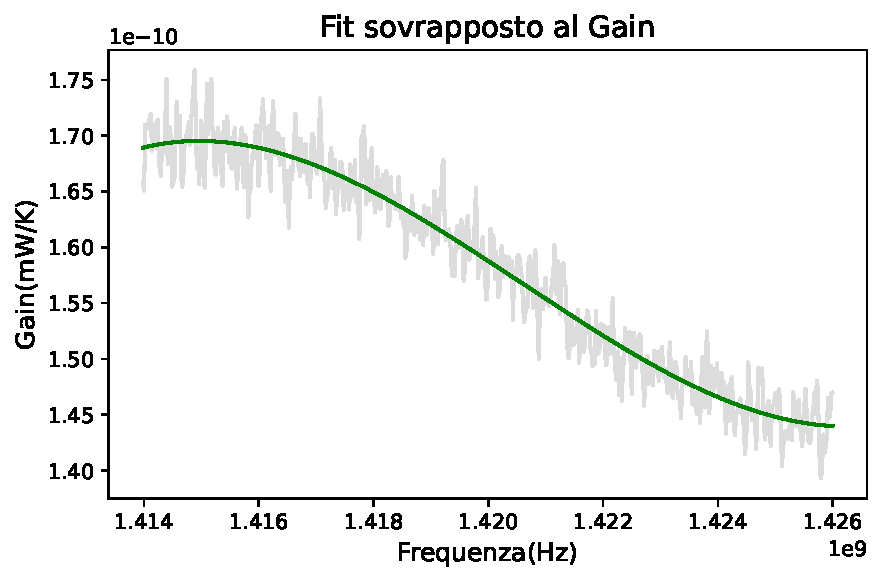
\includegraphics[scale=0.8]{Fit_Gain.pdf}
	\caption{Sovrapposizione del fit rispetto al gain}
    	\label{fig:Fit_Gain}
\end{figure}

Ottenuto il grafico del gain in funzione della frequenza, si nota una notevole oscillazione del valore, per tale motivo viene esseguito un fit con un polinomio di terzo grado, come riportato in figura \ref{fig:Fit_Gain}.

\subsubsection{Temperatura di rumore}
Si determina, ora, la temperatura di rumore, $T_{R}$, sia per il cavo warm load sia per il cold load utilizzando i valori del gain ottenuti dal fit in figura \ref{fig:Fit_Gain} e i valori di $W_{warm}$ e $W_{cold}$ definiti in \ref{ssec:Guadagno del ricevitore}:
 
\begin{equation}
T_{R} = \dfrac{W_{cold}}{G_{plot}}-T_{cold},
\label{Temperatura rumore cold}
\end{equation}

\begin{equation}
T_{R} = \dfrac{W_{warm}}{G_{plot}}-T_{warm},
\label{Temperatura rumore warm}
\end{equation}

Dove \eqref{Temperatura rumore cold} e \eqref{Temperatura rumore warm} si riferiscono, rispettivamente, alla temperatura di rumore relativa al cavo cold load e al cavo warm load.
Si osserva che il segnale ricavato da \eqref{Temperatura rumore cold} risulta essere meno oscillante rispetto al segnale determinato da \eqref{Temperatura rumore warm}. Si sceglie, di conseguenza, di considerare esclusivamente la temperatura di rumore relativa al cavo cold load.

\begin{figure}[H]
\centering

\begin{subfigure}[h!]{0.49\textwidth}
	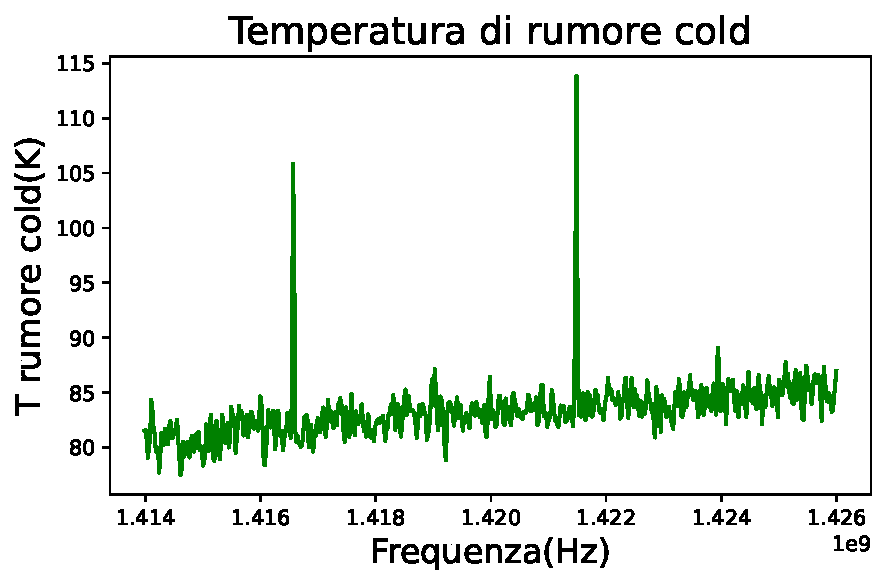
\includegraphics[width=\textwidth]{Temperatura_rumore_cold.pdf}
    \label{fig:sub1}
\end{subfigure}
\hfill
\begin{subfigure}[h!]{0.49\textwidth}
    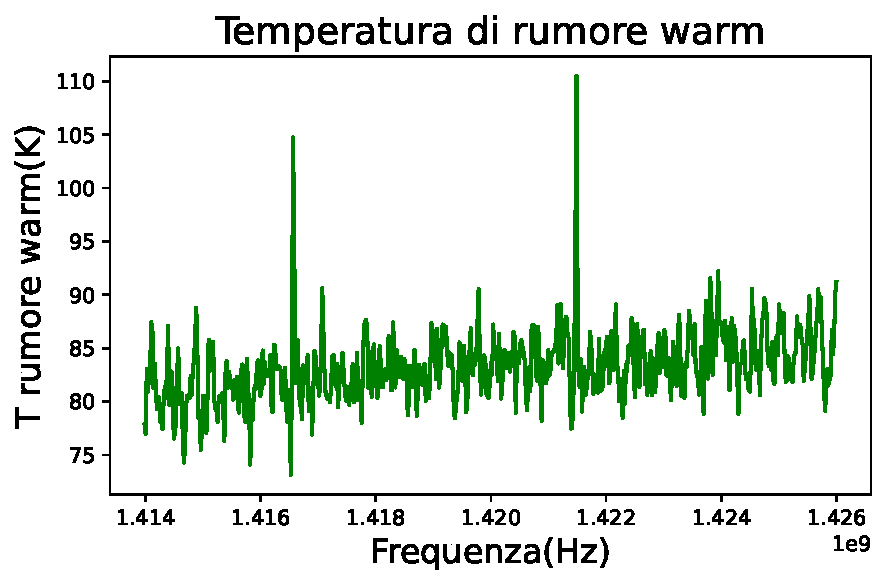
\includegraphics[width=\textwidth]{Temperatura_rumore_warm.pdf}
    \label{fig:sub2}
\end{subfigure}
\caption{Temperature di rumore in funzione della frequenza}
\end{figure}


\subsubsection{Conclusione}
Il procedimento della calibrazione descritto nel suddetto capitolo viene eseguito, sia per quanto riguarda il gain che la tempertura di rumore, per tre set di dati differenti campionati a 5 minuti di distanza l'uno dall'altro. Per ogni set di dati si è scelto di considerare solamente i dati ricavati da \eqref{ssec:Temperatura del cavo cold load}.\\
I tre set di dati vengono prima mediati tra loro, successivamente viene attuata una media mobile ed infine viene eseguito un fit con un polinomio di primo grado. Per quanto concerne i tre valori dei gain, essi vengono semplicemente mediati. 

\begin{figure}[H]
\centering

\begin{subfigure}[h!]{0.49\textwidth}
	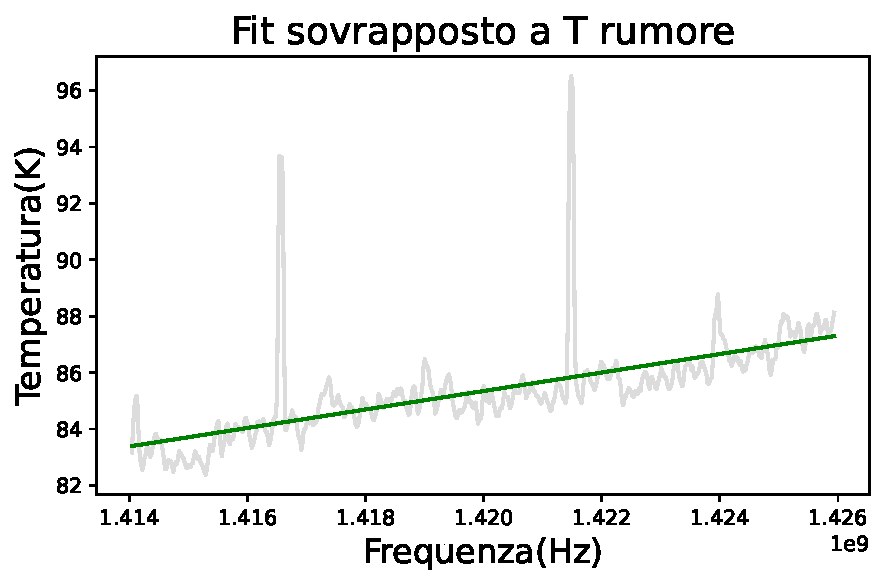
\includegraphics[width=\textwidth]{Fit_T_rumore.pdf}
	\caption{Fit della temperatura di rumore}
    \label{fig:sub1}
\end{subfigure}
\hfill
\begin{subfigure}[h!]{0.49\textwidth}
    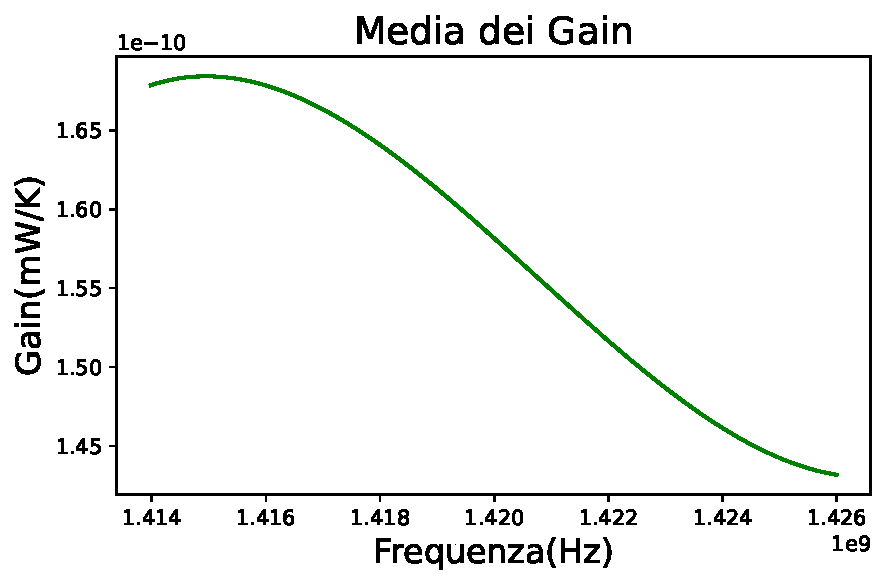
\includegraphics[width=\textwidth]{Media_Gain.pdf}
    \caption{Media tra i Gain}
    \label{fig:sub2}
\end{subfigure}
\end{figure}



I valori finali ottenuti per il guadagno e per $T_{R}$ saranno utilizzati nel calcolo della temperatura di brillanza.






	\section{Analisi Dati e Velocità}
\label{Analisi Dati e Velocità}



\subsection{}
	\section{Mappa}

Viene discussa ora la realizzazione della mappa di una regione di cielo, in corrispondenza del cigno. L'attenzione è posta nell'intervallo di valori tra 38 e 47 deg di declinazione (Dec), e 290 e 320 deg di ascensione retta (RA).
\\\\
Per ottenere i dati di interesse, ad ogni puntamento della parabole si sceglie di lasciare fisso il valore di declinazione lasciando variare l'ascensione retta. Di conseguenza ciascuna osservazione fornirà una riga orizzontale della mappa. Ripetendo i campionamenti su vari giorni è possibile costruire la mappa completa. 
\\\\
Le coordinate, in azimuth ed elevazione, da fornire alla parabola vengono ricavate utilizzando lo stesso programma descritto in \ref{Programma coordinate}; scegliendo il valore di declinazione giornalmente, ponendo l' RA a 308 $^{\circ}$, valore di coordinata celeste del cigno. Osservazioni della durata di 3:00 h permetto di spaziare sul range di 30 $^{\circ}$ di RA citato precedentemente.



\subsection{Composizione della mappa}

Per ogni osservazione vengono in totale utilizzati 32 file, le rispettive coordinate azimuth ed elevazione sono sempre ricavabili sfruttando la funzione $transform_to$. Per ogni file viene eseguita l'analisi delle velocità descritta nella sezione \ref{Analisi Dati e Velocità}. D'interesse è il valore della temperatura di brillanza in corrispondenza del primo picco osservato. 
\\\\
Analizzando ognuno dei set di dati, si possono comporre le varie righe, corrispondenti a declinazioni diverse, attraverso la funzione di stampa $\textit{imshow}$, presenta nella libreria $\textit{mathplotlib}$ di python. Nel dettaglio, è possibile passare, come argomento della funzione, la variabile $\textit{extent}$, ovvero le coordinate che compongono la griglia, nel nostro caso [290-308; 38-47].
\\\\
Il risultato finale è qui riportato: 

\begin{figure}[H]
	\centering
	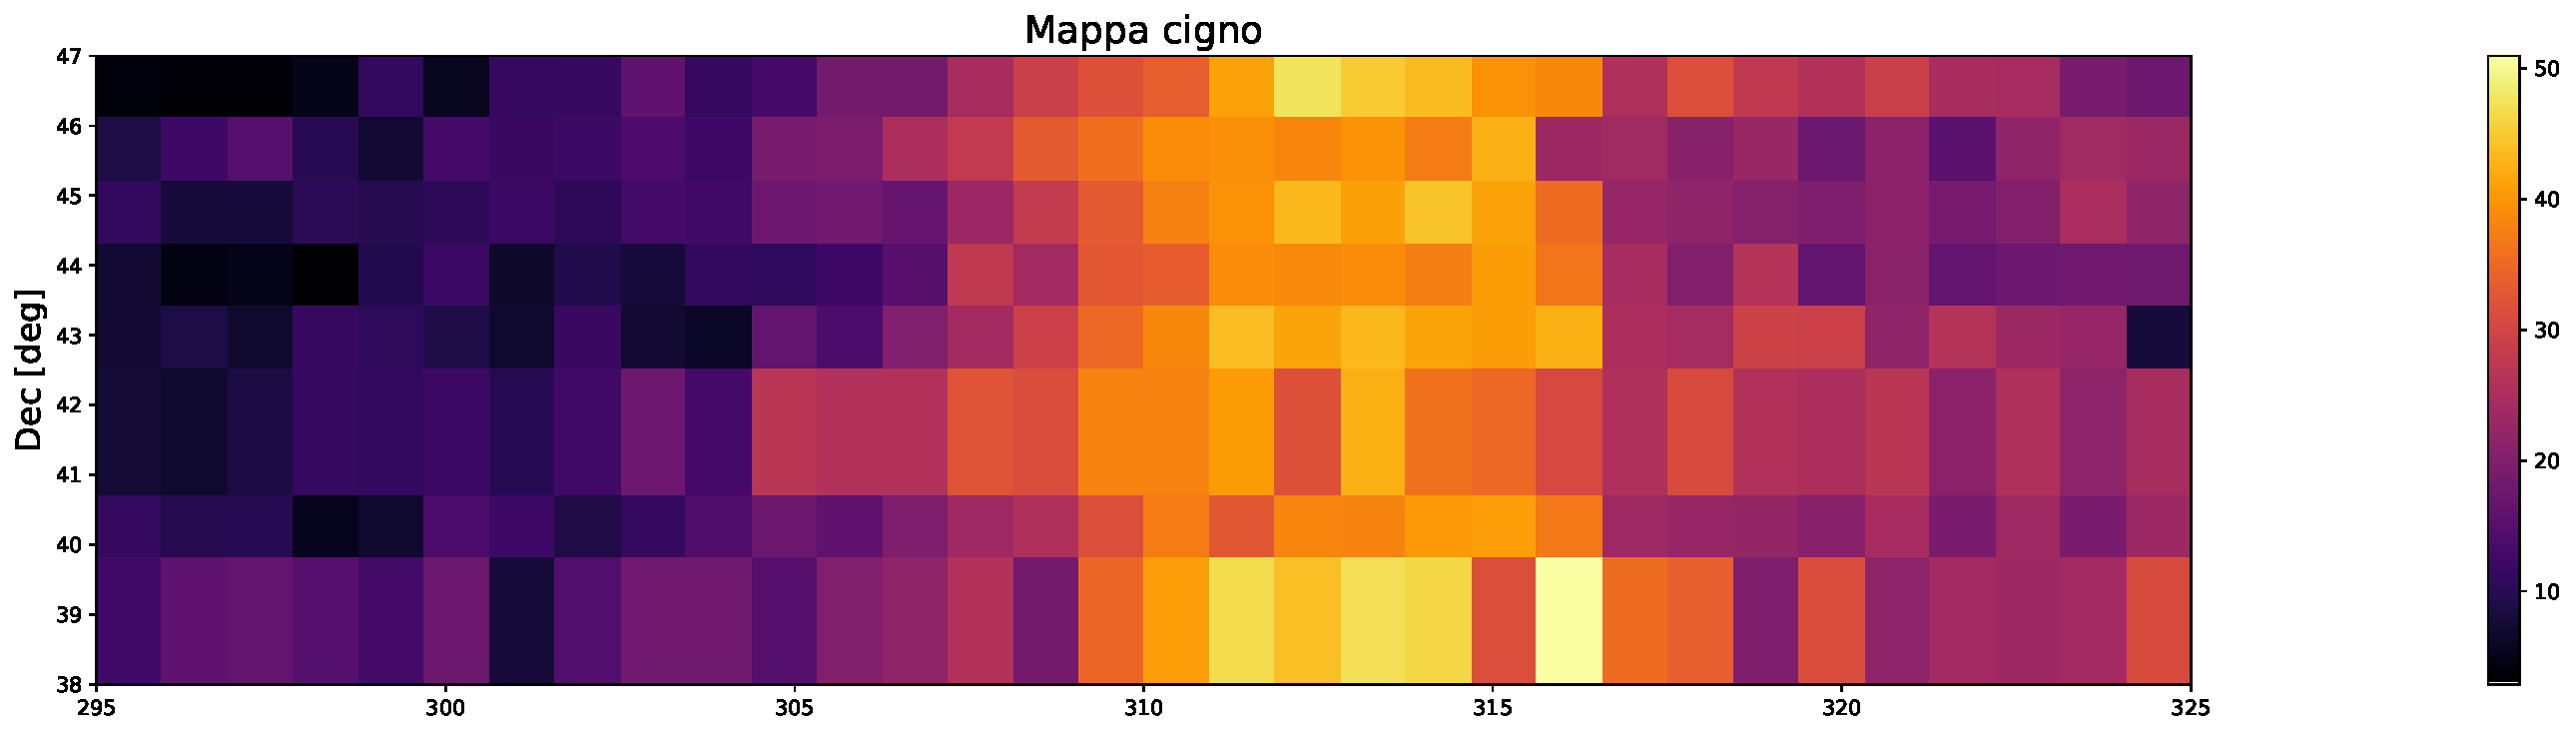
\includegraphics[scale=0.4]{Mappa_grezza.pdf}
	\caption{Mappa del cigno, le intensità dei colori corrispondo ai valori della temperatura di brillanza come indicato nella barra a lato espressa in Kelvin}
    	\label{fig:Mappa_grezza}
\end{figure}

\subsection{Processo di smoothing della mappa}

Il risultato ottenuto, mostrato in figura \ref{fig:Mappa_grezza}, è notevolmente grezzo e irregolare. Per tale motivazione, viene attenuata una procedura di smoothing della mappa, al fine di ottenere un risultato continuo ed uniforme.
\\\\
La procedura si dipana in due passaggi. Il primo step consiste nell'applicare una convoluzione tra il set di dati e un kernel gaussiano bidimensionale. Ci si avvale direttamente della funzione $\textit{convolve}$ ottenendo la seguente mappa:

\begin{figure}[H]
	\centering
	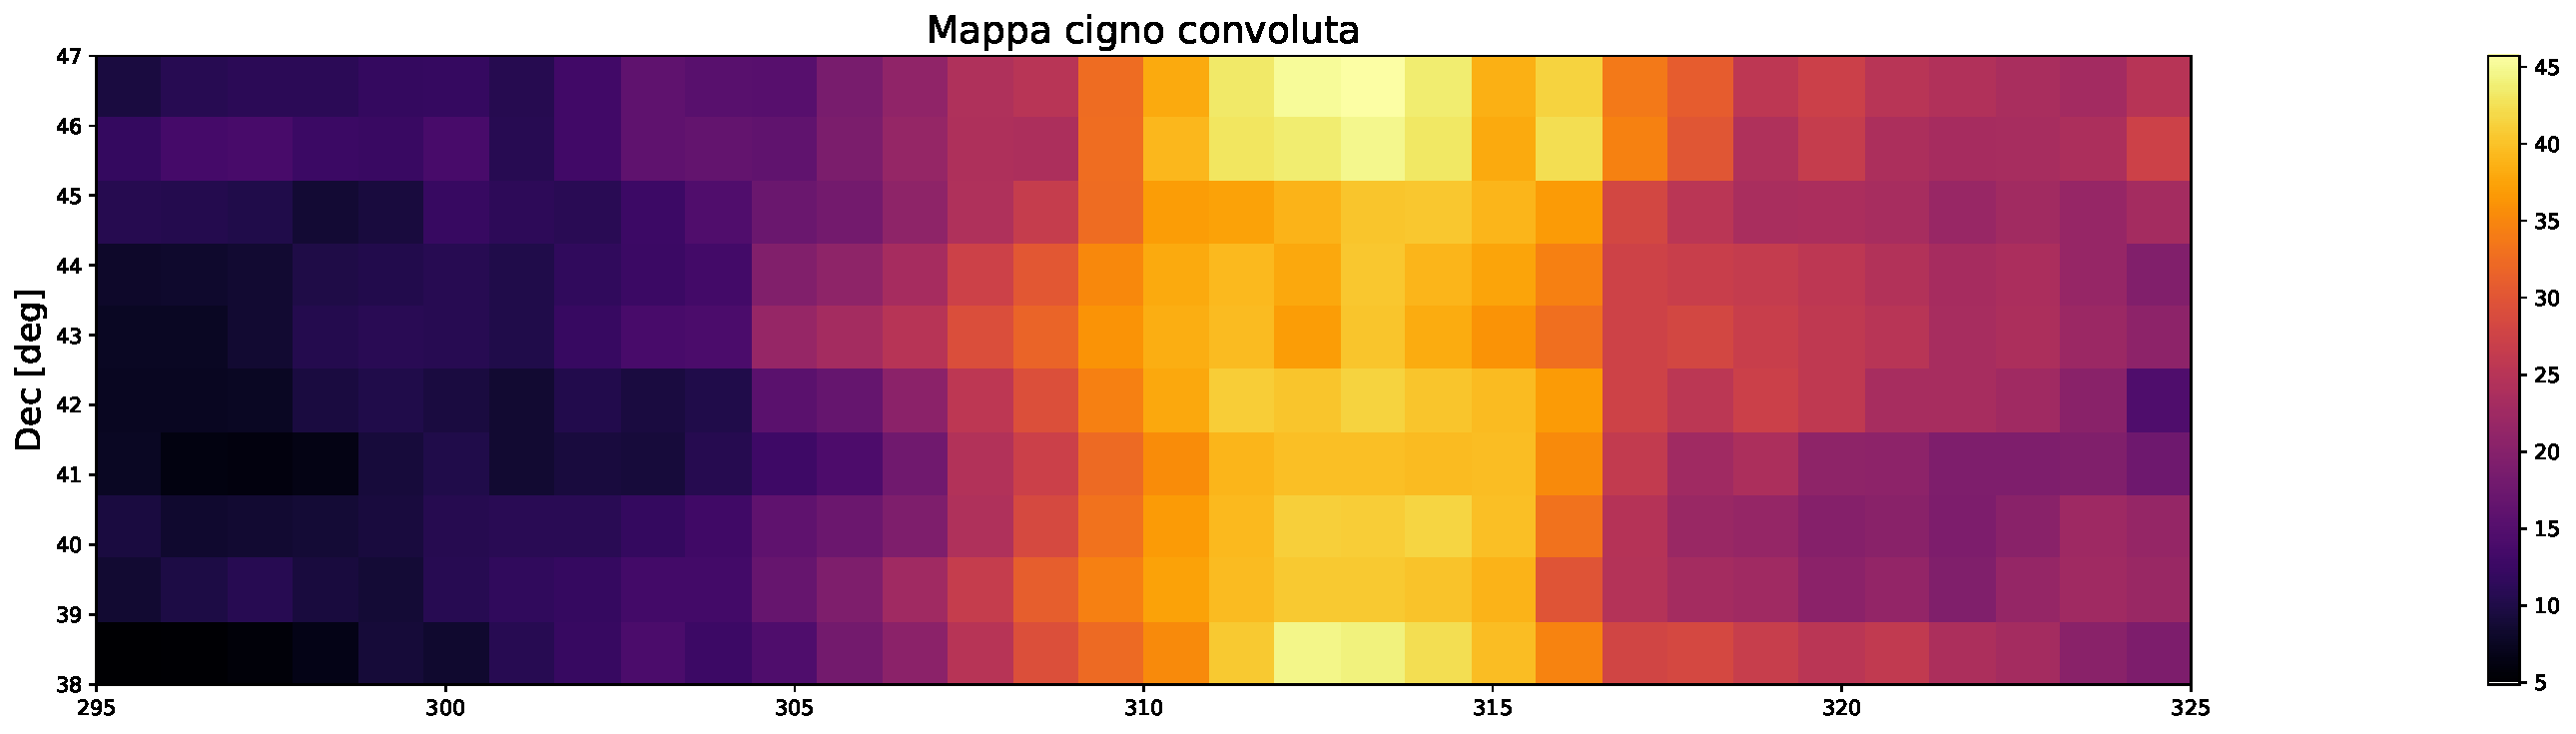
\includegraphics[scale=0.4]{Mappa_convolve.pdf}
	\caption{Mappa del cigno convoluta con un kernel gaussiano}
    	\label{fig:Mappa_convolve}
\end{figure}

Si può notare un minor distacco tra i colori, i.e. temperatura, associati ai diversi pixel.
\\\\
Il secondo step ha il fine di rimuovere il distacco dato dalla griglia dei pixel passando a un andamento maggiormente omogeneo. La già utilizzata funzione $\textit{imshow}$ permette di eseguire un'interpolazione tra un pixel e i suoi adiacenti. Viene qui riportato la mappa finale, ottenibile interpolando le funzioni di Bessel; 

\begin{figure}[H]
	\centering
	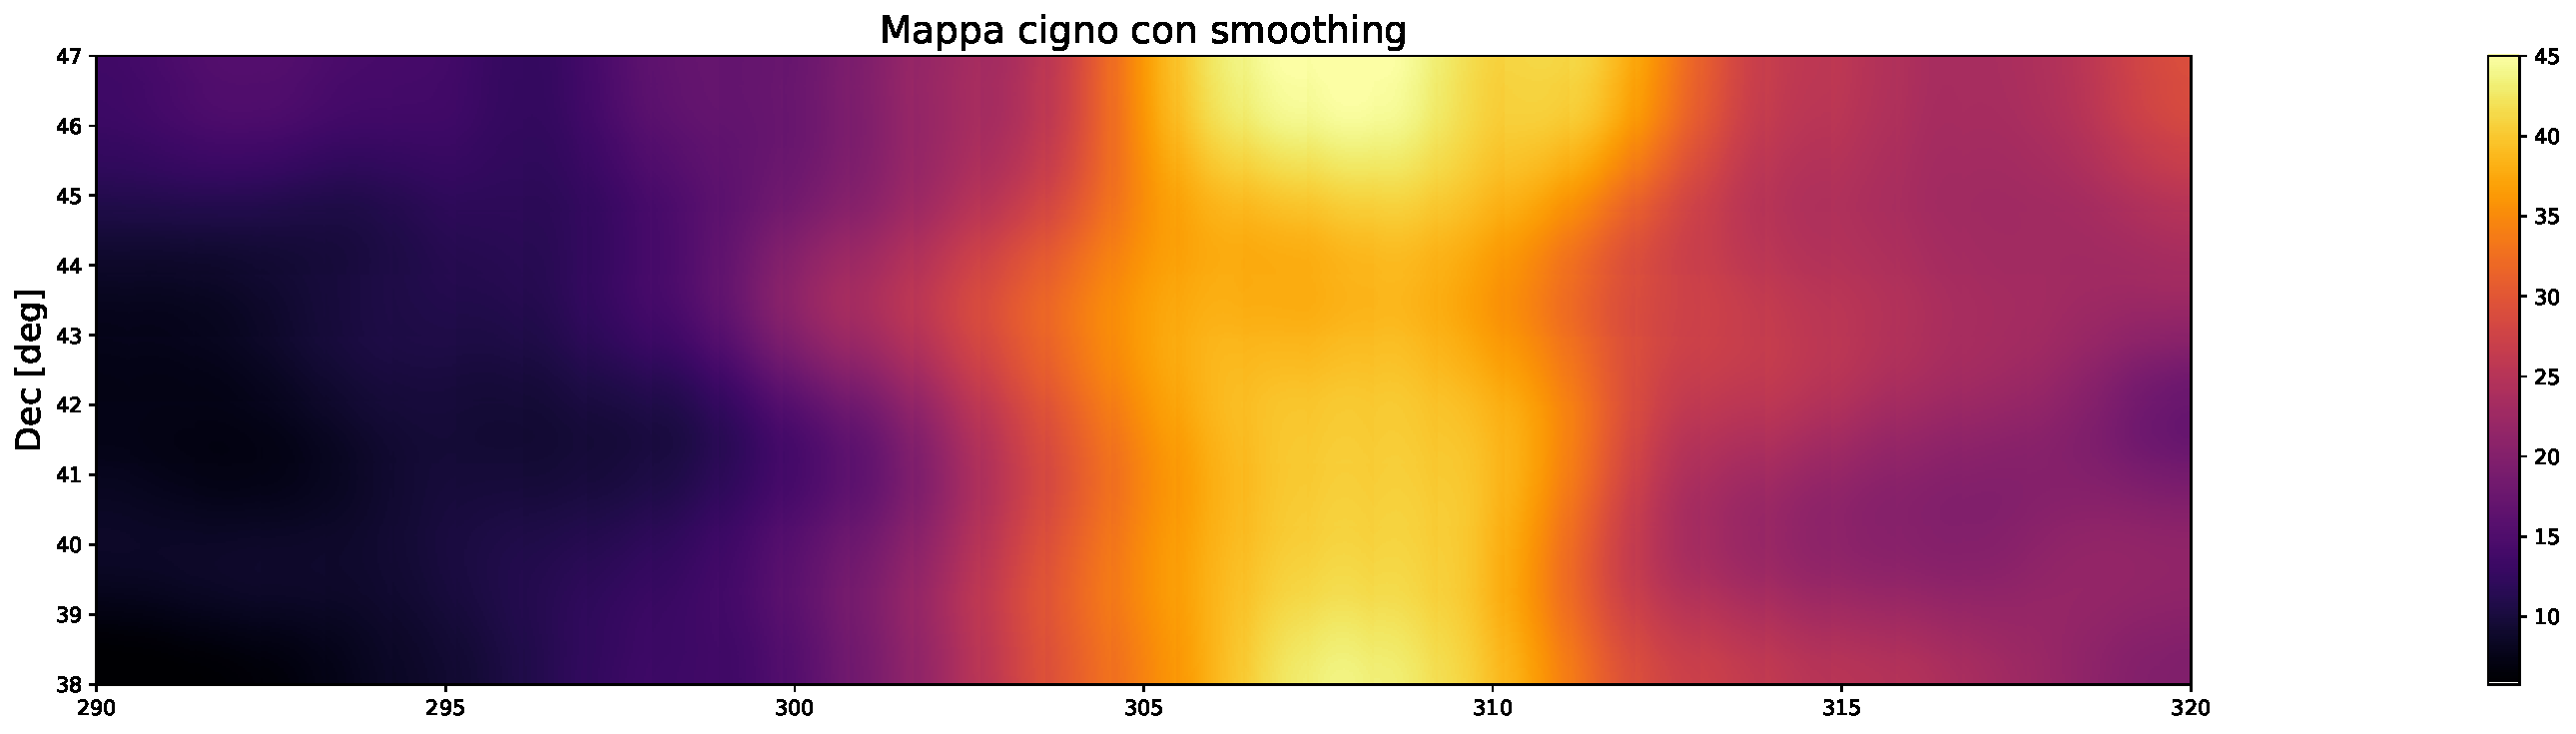
\includegraphics[scale=0.4]{Mappa_finale.pdf}
	\caption{Mappa del cigno a cui è stato applicato il processo di smoothing}
    	\label{fig:Mappa_finale}
\end{figure}

Si noti la corrispondenza tra i punti in cui sono presenti i valori maggiori di temperatura di brillanza e le coordinate galattiche della regione del cigno, fulcro dello studio eseguito.



	\section{Conclusione}

Gli obiettivi prefissati all'inizio dell'esperienza sono stati raggiunti con successo. Lo studio della calibrazione ha permesso di valutare quantitativamente il contributo della strumentazione utilizzata durante la presa dei set di dati, nel corso dell'esperienza.
\\\\
Un corretto svolgimento di essa ha portato a una soddisfacente analisi  riguardante la regione dell'idrogeno, in particolare l'emissione della riga H21.
I risultati finali sono stati ottenuti tenendo conto delle considerazioni sull'effetto Doppler e sul moto di rivoluzione terrestre.
\\\\
Mettici 30 e Lode grazi tesoro.

\begin{figure}[H]
	\centering
	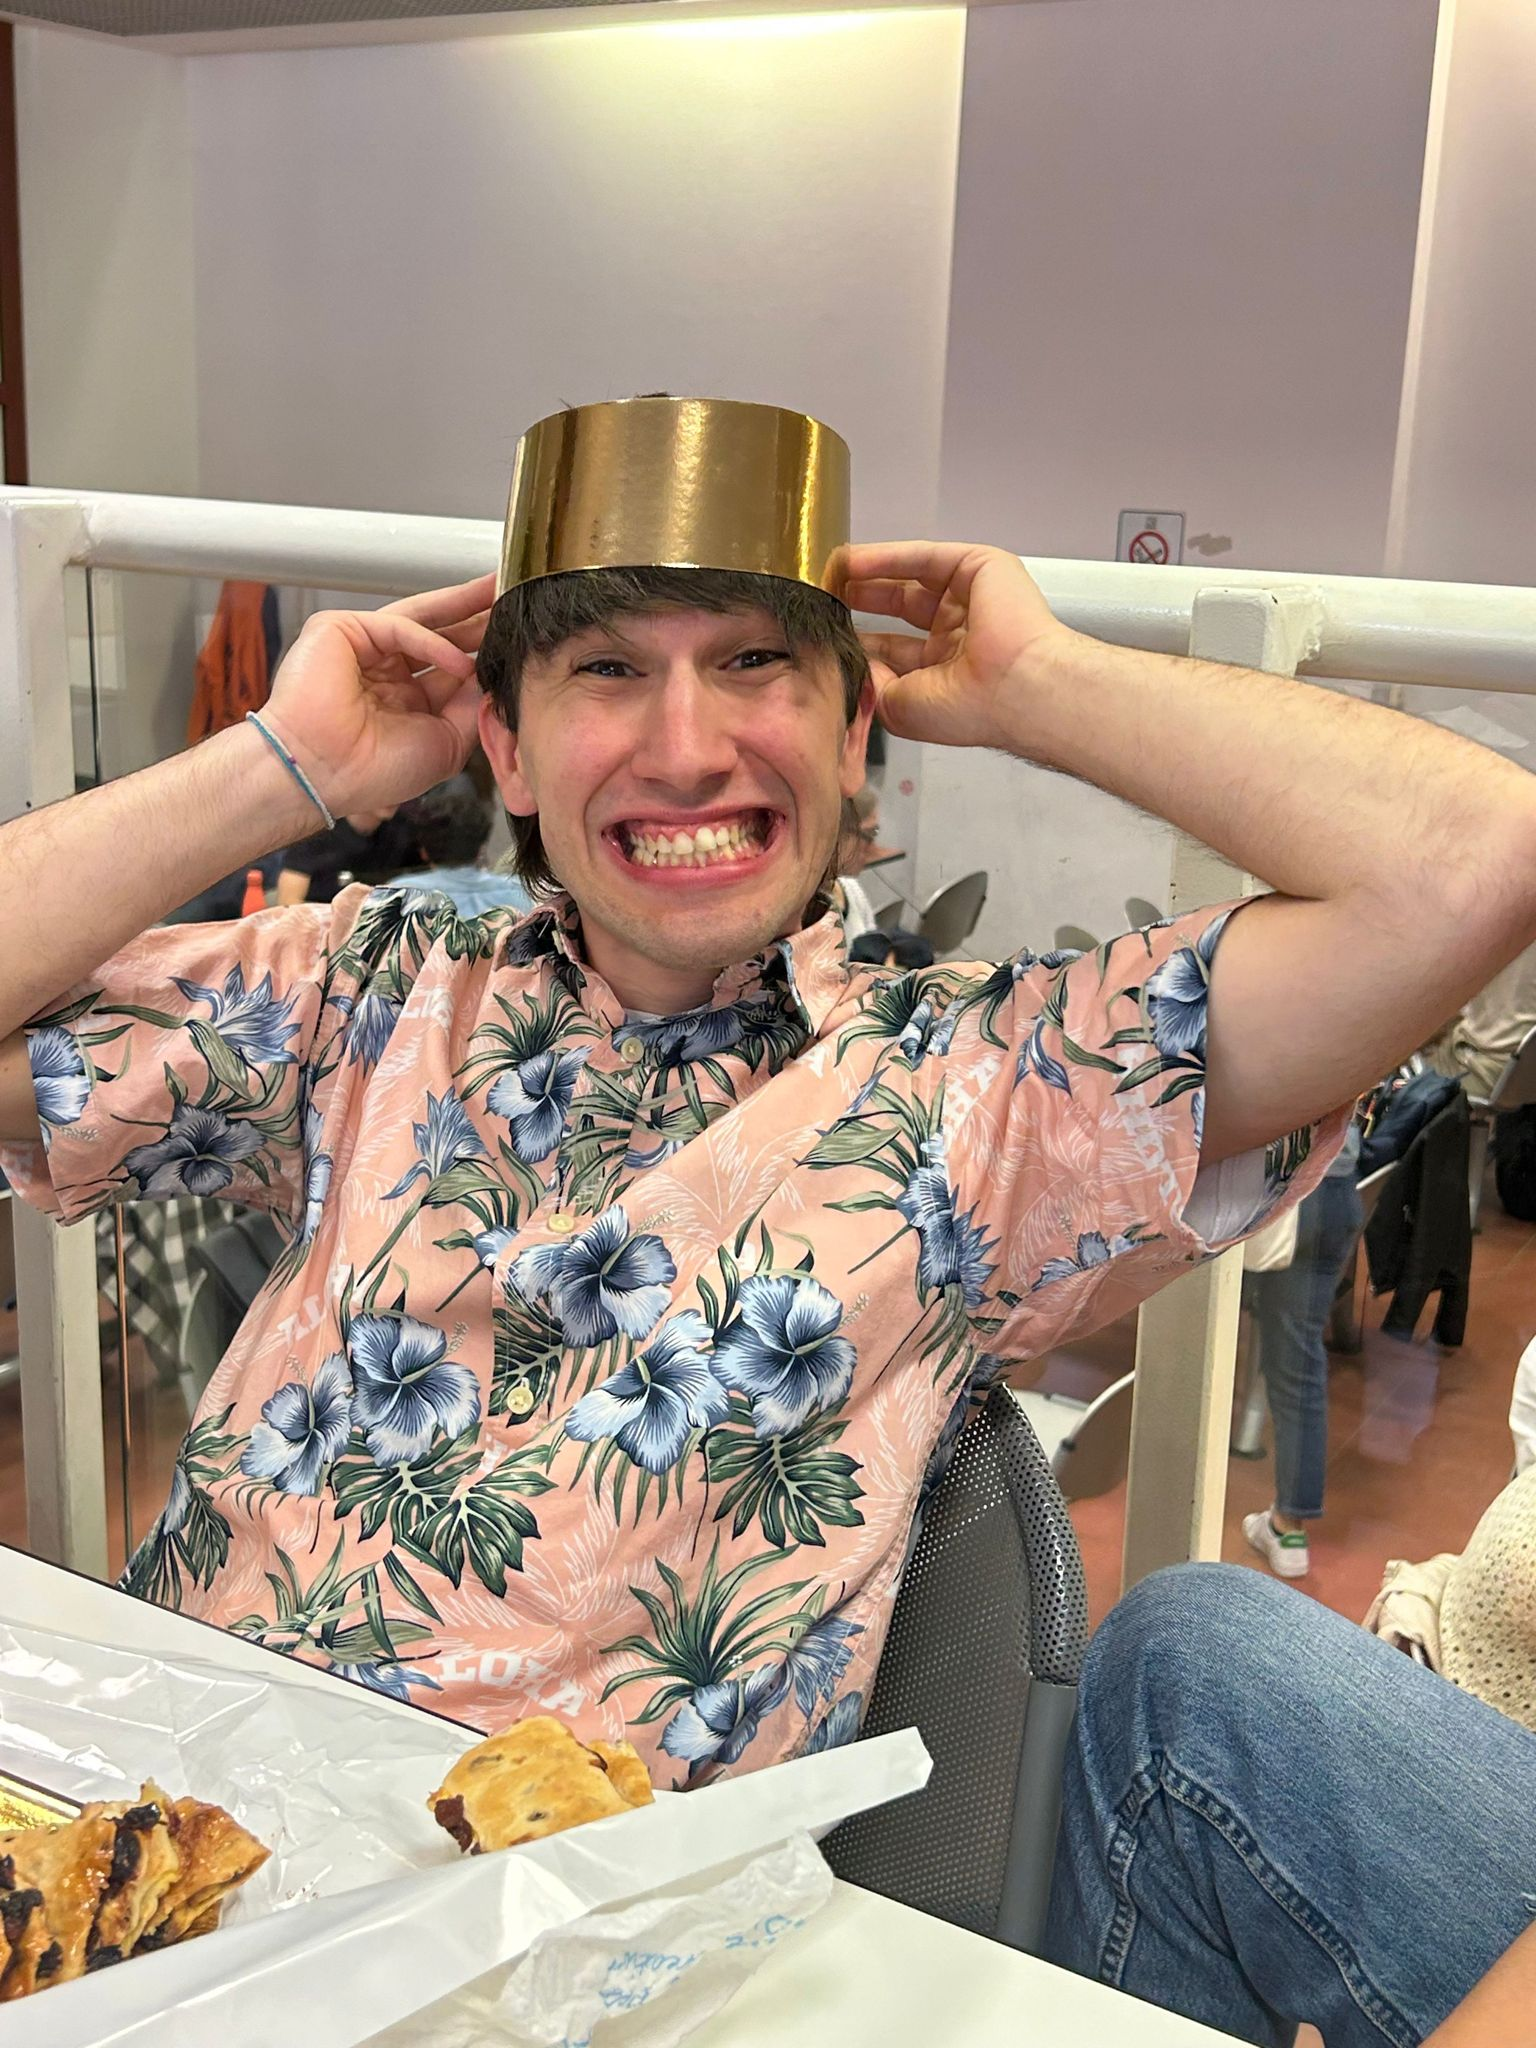
\includegraphics[scale=0.1]{Mapp_cigno_2.jpeg}
	\caption{Il nostro Cigno}
    	\label{fig:Mappa_finale}
\end{figure}  
	
	%\bibliographystyle{plain}
	\printbibliography   
	   
\end{document}
        